\documentclass[]{article}
\usepackage{lmodern}
\usepackage{amssymb,amsmath}
\usepackage{ifxetex,ifluatex}
\usepackage{fixltx2e} % provides \textsubscript
\ifnum 0\ifxetex 1\fi\ifluatex 1\fi=0 % if pdftex
  \usepackage[T1]{fontenc}
  \usepackage[utf8]{inputenc}
\else % if luatex or xelatex
  \ifxetex
    \usepackage{mathspec}
  \else
    \usepackage{fontspec}
  \fi
  \defaultfontfeatures{Ligatures=TeX,Scale=MatchLowercase}
\fi
% use upquote if available, for straight quotes in verbatim environments
\IfFileExists{upquote.sty}{\usepackage{upquote}}{}
% use microtype if available
\IfFileExists{microtype.sty}{%
\usepackage{microtype}
\UseMicrotypeSet[protrusion]{basicmath} % disable protrusion for tt fonts
}{}
\usepackage[margin=1in]{geometry}
\usepackage{hyperref}
\hypersetup{unicode=true,
            pdftitle={随机模拟方法与应用导论 作业四},
            pdfauthor={陈稼霖 45875852},
            pdfborder={0 0 0},
            breaklinks=true}
\urlstyle{same}  % don't use monospace font for urls
\usepackage{color}
\usepackage{fancyvrb}
\newcommand{\VerbBar}{|}
\newcommand{\VERB}{\Verb[commandchars=\\\{\}]}
\DefineVerbatimEnvironment{Highlighting}{Verbatim}{commandchars=\\\{\}}
% Add ',fontsize=\small' for more characters per line
\usepackage{framed}
\definecolor{shadecolor}{RGB}{248,248,248}
\newenvironment{Shaded}{\begin{snugshade}}{\end{snugshade}}
\newcommand{\AlertTok}[1]{\textcolor[rgb]{0.94,0.16,0.16}{#1}}
\newcommand{\AnnotationTok}[1]{\textcolor[rgb]{0.56,0.35,0.01}{\textbf{\textit{#1}}}}
\newcommand{\AttributeTok}[1]{\textcolor[rgb]{0.77,0.63,0.00}{#1}}
\newcommand{\BaseNTok}[1]{\textcolor[rgb]{0.00,0.00,0.81}{#1}}
\newcommand{\BuiltInTok}[1]{#1}
\newcommand{\CharTok}[1]{\textcolor[rgb]{0.31,0.60,0.02}{#1}}
\newcommand{\CommentTok}[1]{\textcolor[rgb]{0.56,0.35,0.01}{\textit{#1}}}
\newcommand{\CommentVarTok}[1]{\textcolor[rgb]{0.56,0.35,0.01}{\textbf{\textit{#1}}}}
\newcommand{\ConstantTok}[1]{\textcolor[rgb]{0.00,0.00,0.00}{#1}}
\newcommand{\ControlFlowTok}[1]{\textcolor[rgb]{0.13,0.29,0.53}{\textbf{#1}}}
\newcommand{\DataTypeTok}[1]{\textcolor[rgb]{0.13,0.29,0.53}{#1}}
\newcommand{\DecValTok}[1]{\textcolor[rgb]{0.00,0.00,0.81}{#1}}
\newcommand{\DocumentationTok}[1]{\textcolor[rgb]{0.56,0.35,0.01}{\textbf{\textit{#1}}}}
\newcommand{\ErrorTok}[1]{\textcolor[rgb]{0.64,0.00,0.00}{\textbf{#1}}}
\newcommand{\ExtensionTok}[1]{#1}
\newcommand{\FloatTok}[1]{\textcolor[rgb]{0.00,0.00,0.81}{#1}}
\newcommand{\FunctionTok}[1]{\textcolor[rgb]{0.00,0.00,0.00}{#1}}
\newcommand{\ImportTok}[1]{#1}
\newcommand{\InformationTok}[1]{\textcolor[rgb]{0.56,0.35,0.01}{\textbf{\textit{#1}}}}
\newcommand{\KeywordTok}[1]{\textcolor[rgb]{0.13,0.29,0.53}{\textbf{#1}}}
\newcommand{\NormalTok}[1]{#1}
\newcommand{\OperatorTok}[1]{\textcolor[rgb]{0.81,0.36,0.00}{\textbf{#1}}}
\newcommand{\OtherTok}[1]{\textcolor[rgb]{0.56,0.35,0.01}{#1}}
\newcommand{\PreprocessorTok}[1]{\textcolor[rgb]{0.56,0.35,0.01}{\textit{#1}}}
\newcommand{\RegionMarkerTok}[1]{#1}
\newcommand{\SpecialCharTok}[1]{\textcolor[rgb]{0.00,0.00,0.00}{#1}}
\newcommand{\SpecialStringTok}[1]{\textcolor[rgb]{0.31,0.60,0.02}{#1}}
\newcommand{\StringTok}[1]{\textcolor[rgb]{0.31,0.60,0.02}{#1}}
\newcommand{\VariableTok}[1]{\textcolor[rgb]{0.00,0.00,0.00}{#1}}
\newcommand{\VerbatimStringTok}[1]{\textcolor[rgb]{0.31,0.60,0.02}{#1}}
\newcommand{\WarningTok}[1]{\textcolor[rgb]{0.56,0.35,0.01}{\textbf{\textit{#1}}}}
\usepackage{graphicx,grffile}
\makeatletter
\def\maxwidth{\ifdim\Gin@nat@width>\linewidth\linewidth\else\Gin@nat@width\fi}
\def\maxheight{\ifdim\Gin@nat@height>\textheight\textheight\else\Gin@nat@height\fi}
\makeatother
% Scale images if necessary, so that they will not overflow the page
% margins by default, and it is still possible to overwrite the defaults
% using explicit options in \includegraphics[width, height, ...]{}
\setkeys{Gin}{width=\maxwidth,height=\maxheight,keepaspectratio}
\IfFileExists{parskip.sty}{%
\usepackage{parskip}
}{% else
\setlength{\parindent}{0pt}
\setlength{\parskip}{6pt plus 2pt minus 1pt}
}
\setlength{\emergencystretch}{3em}  % prevent overfull lines
\providecommand{\tightlist}{%
  \setlength{\itemsep}{0pt}\setlength{\parskip}{0pt}}
\setcounter{secnumdepth}{0}
% Redefines (sub)paragraphs to behave more like sections
\ifx\paragraph\undefined\else
\let\oldparagraph\paragraph
\renewcommand{\paragraph}[1]{\oldparagraph{#1}\mbox{}}
\fi
\ifx\subparagraph\undefined\else
\let\oldsubparagraph\subparagraph
\renewcommand{\subparagraph}[1]{\oldsubparagraph{#1}\mbox{}}
\fi

%%% Use protect on footnotes to avoid problems with footnotes in titles
\let\rmarkdownfootnote\footnote%
\def\footnote{\protect\rmarkdownfootnote}

%%% Change title format to be more compact
\usepackage{titling}

% Create subtitle command for use in maketitle
\providecommand{\subtitle}[1]{
  \posttitle{
    \begin{center}\large#1\end{center}
    }
}

\setlength{\droptitle}{-2em}

  \title{随机模拟方法与应用导论 作业四}
    \pretitle{\vspace{\droptitle}\centering\huge}
  \posttitle{\par}
    \author{陈稼霖 45875852}
    \preauthor{\centering\large\emph}
  \postauthor{\par}
      \predate{\centering\large\emph}
  \postdate{\par}
    \date{2019-10-02}

\usepackage[UTF8]{ctex}

\begin{document}
\maketitle

\hypertarget{drawing-houses}{%
\section{4.5 (Drawing houses)}\label{drawing-houses}}

The following function house plots an outline of a house centered about
the point \texttt{(x,\ y)}:

\begin{verbatim}
house=function(x, y, ...){
lines(c(x - 1, x + 1, x + 1, x - 1, x - 1),
c(y - 1, y - 1, y + 1, y + 1, y - 1), ...)
lines(c(x - 1, x, x + 1), c(y + 1, y + 2, y + 1), ...)
lines(c(x - 0.3, x + 0.3, x + 0.3, x - 0.3, x - 0.3),
c(y - 1, y - 1, y + 0.4, y + 0.4, y - 1), ...)
}
\end{verbatim}

\begin{enumerate}
\def\labelenumi{\alph{enumi}.}
\item
  Read the function house into R.
\item
  Use the \texttt{plot.new} function to open a new plot window. Using
  the \texttt{plot.window} function, set up a coordinate system where
  the horizontal and vertical scales both range from \(0\) to \(10\).
\item
  Using three applications of the function house, draw three houses on
  the current plot window centered at the locations \((1, 1)\),
  \((4, 2)\), and \((7, 6)\).
\item
  Using the \texttt{...} argument, one is able to pass along parameters
  that modify attributes of the \texttt{line} function. For example, if
  one was interested in drawing a red house using thick lines at the
  location \((2, 7)\), one can type
\end{enumerate}

\begin{verbatim}
house(2, 7, col="red", lwd=3)
\end{verbatim}

Using the \texttt{col} and \texttt{lty} arguments, draw three additional
houses on the current plot window at different locations, colors, and
line types.

\begin{enumerate}
\def\labelenumi{\alph{enumi}.}
\setcounter{enumi}{4}
\tightlist
\item
  Draw a boundary \texttt{box} about the current plot window using the
  box function.
\end{enumerate}

\begin{enumerate}
\def\labelenumi{\alph{enumi}.}
\tightlist
\item
  将上述方程读入R
\end{enumerate}

\begin{Shaded}
\begin{Highlighting}[]
\NormalTok{house=}\ControlFlowTok{function}\NormalTok{(x, y, ...)\{}
\KeywordTok{lines}\NormalTok{(}\KeywordTok{c}\NormalTok{(x }\OperatorTok{-}\StringTok{ }\DecValTok{1}\NormalTok{, x }\OperatorTok{+}\StringTok{ }\DecValTok{1}\NormalTok{, x }\OperatorTok{+}\StringTok{ }\DecValTok{1}\NormalTok{, x }\OperatorTok{-}\StringTok{ }\DecValTok{1}\NormalTok{, x }\OperatorTok{-}\StringTok{ }\DecValTok{1}\NormalTok{),}
\KeywordTok{c}\NormalTok{(y }\OperatorTok{-}\StringTok{ }\DecValTok{1}\NormalTok{, y }\OperatorTok{-}\StringTok{ }\DecValTok{1}\NormalTok{, y }\OperatorTok{+}\StringTok{ }\DecValTok{1}\NormalTok{, y }\OperatorTok{+}\StringTok{ }\DecValTok{1}\NormalTok{, y }\OperatorTok{-}\StringTok{ }\DecValTok{1}\NormalTok{), ...)}
\KeywordTok{lines}\NormalTok{(}\KeywordTok{c}\NormalTok{(x }\OperatorTok{-}\StringTok{ }\DecValTok{1}\NormalTok{, x, x }\OperatorTok{+}\StringTok{ }\DecValTok{1}\NormalTok{), }\KeywordTok{c}\NormalTok{(y }\OperatorTok{+}\StringTok{ }\DecValTok{1}\NormalTok{, y }\OperatorTok{+}\StringTok{ }\DecValTok{2}\NormalTok{, y }\OperatorTok{+}\StringTok{ }\DecValTok{1}\NormalTok{), ...)}
\KeywordTok{lines}\NormalTok{(}\KeywordTok{c}\NormalTok{(x }\OperatorTok{-}\StringTok{ }\FloatTok{0.3}\NormalTok{, x }\OperatorTok{+}\StringTok{ }\FloatTok{0.3}\NormalTok{, x }\OperatorTok{+}\StringTok{ }\FloatTok{0.3}\NormalTok{, x }\OperatorTok{-}\StringTok{ }\FloatTok{0.3}\NormalTok{, x }\OperatorTok{-}\StringTok{ }\FloatTok{0.3}\NormalTok{),}
\KeywordTok{c}\NormalTok{(y }\OperatorTok{-}\StringTok{ }\DecValTok{1}\NormalTok{, y }\OperatorTok{-}\StringTok{ }\DecValTok{1}\NormalTok{, y }\OperatorTok{+}\StringTok{ }\FloatTok{0.4}\NormalTok{, y }\OperatorTok{+}\StringTok{ }\FloatTok{0.4}\NormalTok{, y }\OperatorTok{-}\StringTok{ }\DecValTok{1}\NormalTok{), ...)}
\NormalTok{\}}
\end{Highlighting}
\end{Shaded}

\begin{enumerate}
\def\labelenumi{\alph{enumi}.}
\setcounter{enumi}{1}
\tightlist
\item
  用\texttt{plot.new}函数新建一个绘图窗口,然后用\texttt{plot.window}函数设定横纵范围均为\(0\)到\(10\)的坐标系
\end{enumerate}

\begin{Shaded}
\begin{Highlighting}[]
\KeywordTok{plot.new}\NormalTok{()}
\end{Highlighting}
\end{Shaded}


\includegraphics{Homework_4_files/figure-latex/unnamed-chunk-2-1.pdf}

\begin{Shaded}
\begin{Highlighting}[]
\KeywordTok{plot.window}\NormalTok{(}\DataTypeTok{xlim =} \KeywordTok{c}\NormalTok{(}\DecValTok{0}\NormalTok{,}\DecValTok{10}\NormalTok{),}\DataTypeTok{ylim =} \KeywordTok{c}\NormalTok{(}\DecValTok{0}\NormalTok{,}\DecValTok{10}\NormalTok{))}
\end{Highlighting}
\end{Shaded}

\begin{enumerate}
\def\labelenumi{\alph{enumi}.}
\setcounter{enumi}{2}
\tightlist
\item
  用上面定义的\texttt{house}函数绘制三个中心分别在\((1,1)\),\((4,2)\)和\((7, 6)\)的房子
\end{enumerate}

\begin{Shaded}
\begin{Highlighting}[]
\KeywordTok{plot.new}\NormalTok{()}
\KeywordTok{plot.window}\NormalTok{(}\DataTypeTok{xlim =} \KeywordTok{c}\NormalTok{(}\DecValTok{0}\NormalTok{,}\DecValTok{10}\NormalTok{),}\DataTypeTok{ylim =} \KeywordTok{c}\NormalTok{(}\DecValTok{0}\NormalTok{,}\DecValTok{10}\NormalTok{))}
\KeywordTok{house}\NormalTok{(}\DecValTok{1}\NormalTok{,}\DecValTok{1}\NormalTok{)}
\KeywordTok{house}\NormalTok{(}\DecValTok{4}\NormalTok{,}\DecValTok{2}\NormalTok{)}
\KeywordTok{house}\NormalTok{(}\DecValTok{7}\NormalTok{,}\DecValTok{6}\NormalTok{)}
\end{Highlighting}
\end{Shaded}

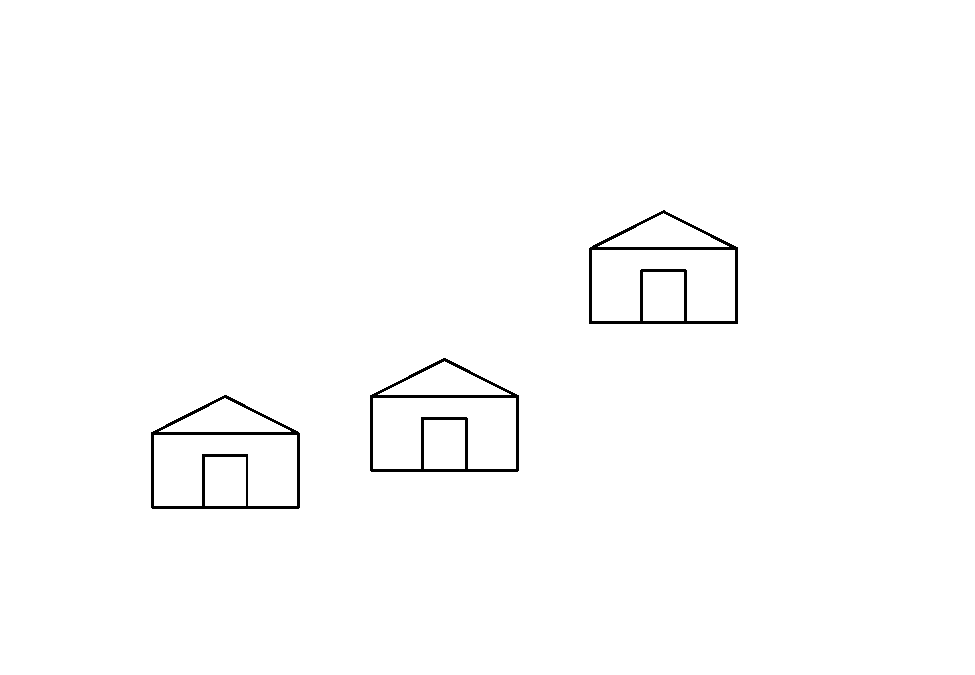
\includegraphics{Homework_4_files/figure-latex/unnamed-chunk-3-1.pdf}

\begin{enumerate}
\def\labelenumi{\alph{enumi}.}
\setcounter{enumi}{3}
\tightlist
\item
  通过向\texttt{...}中输入参数,额外绘制三个具有不同位置、颜色和线条类型的房子
\end{enumerate}

\begin{Shaded}
\begin{Highlighting}[]
\KeywordTok{plot.new}\NormalTok{()}
\KeywordTok{plot.window}\NormalTok{(}\DataTypeTok{xlim =} \KeywordTok{c}\NormalTok{(}\DecValTok{0}\NormalTok{,}\DecValTok{10}\NormalTok{),}\DataTypeTok{ylim =} \KeywordTok{c}\NormalTok{(}\DecValTok{0}\NormalTok{,}\DecValTok{10}\NormalTok{))}
\KeywordTok{house}\NormalTok{(}\DecValTok{1}\NormalTok{,}\DecValTok{1}\NormalTok{)}
\KeywordTok{house}\NormalTok{(}\DecValTok{4}\NormalTok{,}\DecValTok{2}\NormalTok{)}
\KeywordTok{house}\NormalTok{(}\DecValTok{7}\NormalTok{,}\DecValTok{6}\NormalTok{)}
\KeywordTok{house}\NormalTok{(}\DecValTok{1}\NormalTok{,}\DecValTok{5}\NormalTok{,}\DataTypeTok{col =} \StringTok{'red'}\NormalTok{,}\DataTypeTok{lty =} \StringTok{'dashed'}\NormalTok{)}
\KeywordTok{house}\NormalTok{(}\DecValTok{4}\NormalTok{,}\DecValTok{6}\NormalTok{,}\DataTypeTok{col =} \StringTok{'green'}\NormalTok{,}\DataTypeTok{lty =} \StringTok{'dotted'}\NormalTok{)}
\KeywordTok{house}\NormalTok{(}\DecValTok{7}\NormalTok{,}\DecValTok{2}\NormalTok{,}\DataTypeTok{col =} \StringTok{'blue'}\NormalTok{,}\DataTypeTok{lty =} \StringTok{'dotdash'}\NormalTok{)}
\end{Highlighting}
\end{Shaded}

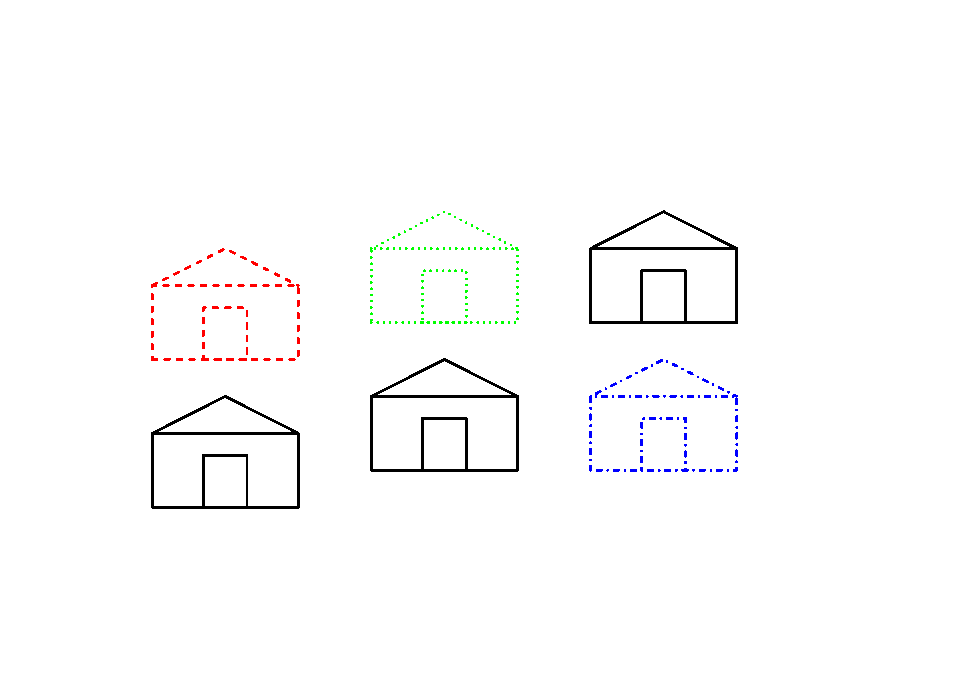
\includegraphics{Homework_4_files/figure-latex/unnamed-chunk-4-1.pdf}

\begin{enumerate}
\def\labelenumi{\alph{enumi}.}
\setcounter{enumi}{4}
\tightlist
\item
  用\texttt{box}函数绘制当前绘图窗口的边界
\end{enumerate}

\begin{Shaded}
\begin{Highlighting}[]
\KeywordTok{plot.new}\NormalTok{()}
\KeywordTok{plot.window}\NormalTok{(}\DataTypeTok{xlim =} \KeywordTok{c}\NormalTok{(}\DecValTok{0}\NormalTok{,}\DecValTok{10}\NormalTok{),}\DataTypeTok{ylim =} \KeywordTok{c}\NormalTok{(}\DecValTok{0}\NormalTok{,}\DecValTok{10}\NormalTok{))}
\KeywordTok{house}\NormalTok{(}\DecValTok{1}\NormalTok{,}\DecValTok{1}\NormalTok{)}
\KeywordTok{house}\NormalTok{(}\DecValTok{4}\NormalTok{,}\DecValTok{2}\NormalTok{)}
\KeywordTok{house}\NormalTok{(}\DecValTok{7}\NormalTok{,}\DecValTok{6}\NormalTok{)}
\KeywordTok{house}\NormalTok{(}\DecValTok{1}\NormalTok{,}\DecValTok{5}\NormalTok{,}\DataTypeTok{col =} \StringTok{'red'}\NormalTok{,}\DataTypeTok{lty =} \StringTok{'dashed'}\NormalTok{)}
\KeywordTok{house}\NormalTok{(}\DecValTok{4}\NormalTok{,}\DecValTok{6}\NormalTok{,}\DataTypeTok{col =} \StringTok{'green'}\NormalTok{,}\DataTypeTok{lty =} \StringTok{'dotted'}\NormalTok{)}
\KeywordTok{house}\NormalTok{(}\DecValTok{7}\NormalTok{,}\DecValTok{2}\NormalTok{,}\DataTypeTok{col =} \StringTok{'blue'}\NormalTok{,}\DataTypeTok{lty =} \StringTok{'dotdash'}\NormalTok{)}
\KeywordTok{box}\NormalTok{()}
\end{Highlighting}
\end{Shaded}

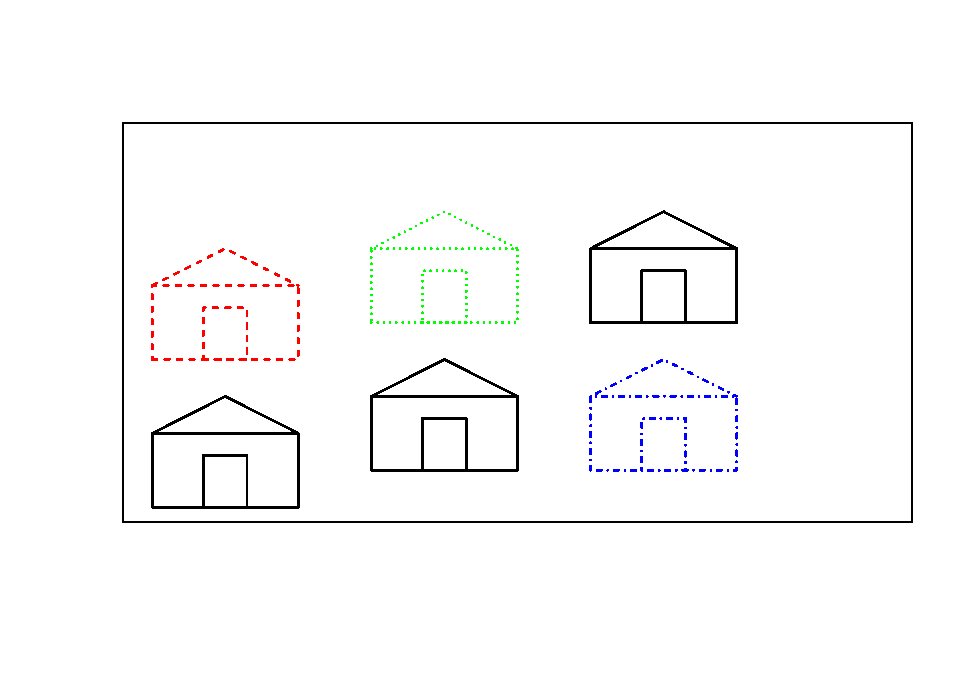
\includegraphics{Homework_4_files/figure-latex/unnamed-chunk-5-1.pdf}


\end{document}
